\section{Bruk av \LaTeX}

\begin{frame}{Introduksjon}
	
	Eit \LaTeX{} dokument består av ein eller fleire kjeldefilar (*.tex) som vanlegvis er reine tekstfilar i UTF-8 format. Filane vert lest av ein \LaTeX{}-kompilator som genererer eit dokument, vanlegivis i *.pdf format.
	
	Programmet (kompilatoren) som les *.tex filane er ein vanleg programfil utan grafisk brukargrensesnitt (eit konsollprogram). Ein har ulike alternativ:
	
	\begin{itemize}
		\item pdflatex
		\item XeLaTeX
		\item LuaLaTeX
	\end{itemize}
	
\end{frame}


\begin{frame}{Introduksjon}

  	\includesvg[width=1in]{img/emacs-logo.svg}
	
	For å redigera kjeldefilane i eit \LaTeX{} dokument treng ein eit tekstredigeringsprogram. Her har ein svært mange å velga mellom (ein kan til og med nytta program som Visual studio, eller Word(!)). TeXstudio er eit program som er speisallaga for å skriva \LaTeX{}, og har ein del innekbygd funksjonalitet for å gjera dette enklare. Emacs er eit anna godt alternativ for dei som allereie nyttar Emacs i andre samanhengar.
	
	I staden for å skriva kommandoen \mintinline{console}|pdflatex bachelorrapport.tex| kan ein trykka på den grøne pilen i TeXstudio for å bygga dokumentet.
	
\end{frame}

\begin{frame}[containsverbatim]{Oppbygging av eit dokument}
	
Kjeldefilen for eit svært enkelt \LaTeX{} dokument kan sjå slik ut:

	\begin{minted}{latex}
\documentclass[10pt,a4paper]{article}
%\usepackage[utf8]{inputenc} % Ikkje for LuaLaTeX
\usepackage[T1]{fontenc}
\usepackage[nynorsk]{babel}

\author{Eirik Haustveit}
\title{Demo}
\begin{document}
	Eit enkelt dokument
\end{document}
	\end{minted}
	
\end{frame}


\begin{frame}[containsverbatim]{Oppbygging av eit dokument}
	
	Koden før \mintinline{latex}|\begin{document}| vert kalla ``preamble''. Her importerer ein pakkar som tilbyr ekstra funksjonalitet og endrar innstillingar som gjeld heile dokumentet.
		
		Mellom \mintinline{latex}|\begin{document}| og \mintinline{latex}|\end{document}| plasserer ein alt innhaldet i dokumentet. Dette inkluderer den reine teksten ein jobbar med, samt kommandoar som markerer teksten for å oppnå dei tilpassingane ein ynskjer.
		
		\mintinline{latex}|\documentclass[10pt,a4paper]{article}| velger dokumentklasse, og setter enkelte innstillingar som gjeld for heile dokumentet. Dette har betydning både for korleis dokumentet ser ut, og kva kommandoar som er tilgjengelig.
		
	\end{frame}

	\begin{frame}[containsverbatim]{Oppbygging av eit dokument}
	

		\mintinline{latex}|\usepackage[utf8]{inputenc}| velger at teksten som \LaTeX{} får inn (den teksten du skriv) skal tolkast som UTF-8. Denne pakken er ikkje nødvendig i dei moderne kompilatorane XeLaTeX, og LuaLaTeX.
		
		\mintinline{latex}|\usepackage[T1]{fontenc}| velger kva type skriftkoding (font encoding) som skal nyttast. Merk at dette ikkje er det samme som å velga skrifttype, det handlar om kva \textit{type} skrifttypar som skal vera tigjengeleg. Denne pakken er nesten alltid med, men ein treng normalt ikkje ta stilling til den. Den \textit{berre er der}.
		
		\mintinline{latex}|\author{Eirik Haustveit}| og \mintinline{latex}|\title{Demo}| vert nytta av ulike verktøy som til dømes kan generera framside automatisk.
		
	\end{frame}
	
	
	\begin{frame}{Inndeling i seksjonar og kapittel}
		
		Inndeling av dokumentet i kapittel og underkapittel (seksjonar) vert gjort med ulike kommandoar avhengig av nivået:
		
		\mintinline{latex}{\section{tittel}}, \mintinline{latex}{\subsection{tittel}}, \mintinline{latex}{\subsubsection{tittel}}
		
		\mintinline{latex}{\chapter{tittel}}
		
		\mintinline{latex}{\part{tittel}}
		
		Det er viktig å ikkje overdriva bruken av slik inndeling. Boka \textit{The Elements of Typographic Style} anbefaler 3 nivå \cite{bringhurstElementsTypographicStyle2002}.
		
	\end{frame}
	
	\begin{frame}{Feilmeldingar}
		
		Dersom du skriv ein ugyldig kommando vil du få ein feilmelding på samme måte som ved kompilering av eit program. Det er ulike kategoriar av feilmeldingar, nokon vil stoppa bygginga av dokumentet, medan andre berre fortel deg at noko er galt og at dokumentet truleg ikkje vil sjå ut slik som du hadde tenkt.
		
		%	\begin{itemize}
			%		\item error
			%		\item warning
			%		\item bad box
			%	\end{itemize}
		
		Det er viktig at ein sjekker feilloggen regelmessig, og at ein håndterer eventuelle feilmeldingar etter kvart. Dersom det hopar seg opp med ``warnings'' så kan det vera mykje arbeid å finna ut av ein feil når det til slutt ikkje fungerer lenger.
		
		\begin{figure}
			\centering
			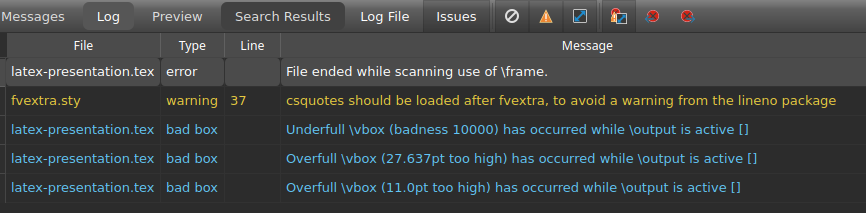
\includegraphics[width=0.9\linewidth]{img/latex-error-example}
			\caption{Døme på feilmeldingar i TeXStudio}
			\label{fig:latex-error-example}
		\end{figure}
		
		
	\end{frame}
	
	\begin{frame}{Dokumentklassar}
		
		\LaTeX{} har ein del innebygde dokumentklassar, og det er også mulig å lasta ned fleire, eller laga sine eigne. Nokon av dei viktigaste er:
		
		\begin{itemize}
			\item article - korte rapportar, dokumentasjon, vitskaplig artikkel m.m.
			\item report - For lengre rapportar, avhandlingar og korte bøker
			\item book - For bøker
			\item letter - For brev
			\item beamer - For presentasjonar (denne presentasjonen er laga i beamer)
		\end{itemize}
		
	\end{frame}




%%% Local Variables:
%%% mode: latex
%%% TeX-master: "../latex-presentation"
%%% End:
